This chapter describes the current status, the measurement principle and the latest updates of the \ac{LND} onboard the lander of Chang`E - 4 mission, and the \ac{HET} onboard \ac{SolO}. 

\section{Chang'E-4 and Lunar Lander Neutron and Dosimetry (LND)Experiment}
\label{sec:change_4_LND}

\subsection*{Overview and current status (2019 - 2022)}

\begin{figure}
    \centering
    \includegraphics[width = 0.9\textwidth]{images/LND_2018-11-13.JPG}
    \caption[A photograph of the \ac{LND}]{A photograph of the \ac{LND}, including the \ac{SH} in the front, \ac{EB} in the rear, and 1-meters data and power harness that connects the \ac{SH} and \ac{EB}. The figure was adapted from \citet{Wimmer2020SSRv} and shows the flight spare model of LND and was taken on 2018.11.23.}
    \label{Fig:LND_instrument}
\end{figure}


\begin{figure}[!htb]
    \centering
    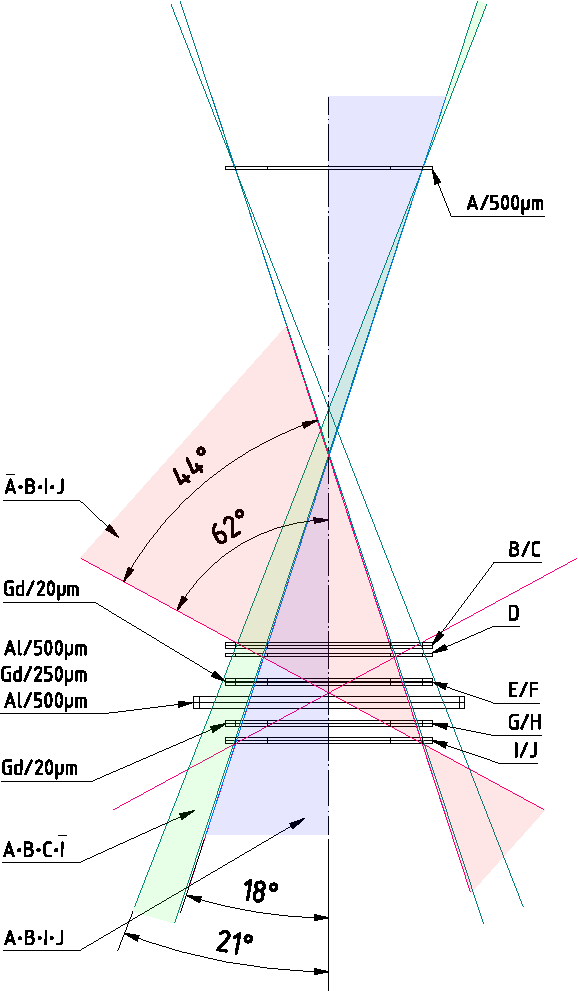
\includegraphics[width = 0.6\textwidth, height = 0.5 \textheight]{images/change4_lnd-c9_trigger-cones-colored.pdf}
    \caption[The inner structure of LND \ac{SH}]{A sketch of the inner structure of the \ac{LND} \ac{SH}. Ten 500 $\mu$m Si \acp{SSD} are assembled in order. The different colored regions indicate the \ac{FOV} of different measurement combinations. The figure was reproduced from \citet{Wimmer2020SSRv}, and more details could be found in the instrument paper.}
    \label{Fig:LND_sensor_head}
\end{figure}
Chang'E-4 is a robotic spacecraft mission of China exploring the lunar far-side surface, which is also the first soft-landing mission on the lunar far-side surface \citep{Li2021SSRv}. The whole mission consists of a lander, a rover named Yutu-2, and a relay satellite named Queqiao which works on a halo orbit around the Earth - Moon L2 Lagrangian point, and enables the communication between the lunar far-side surface and the ground. The mission was launched on December 8, 2018, and successfully landed on the Von K\`arm\`an crater near the south pole of the Moon on January 3, 2019 \citep{Wu2019NatGe}. In order to cope with the significant temperature variations on the lunar surface, the rover, lander, and scientific payloads onboard enter a hibernation state during the approximately two-week-long lunar night, to avoid possible damage caused by the unexpected cold temperature (down to -190 degrees Celsius according to the result from Chang'E-4) on the lunar far-side surface. After the extended 'sleep' night, the probe and the instruments onboard wake up autonomously after they detecting the sunlight, and start regular operation during the lunar daytime. The initial design lifetime of the mission was set at a minimum of one year. Obviously, this target has been successfully surpassed, and the scientific instruments onboard are continuing to perform impressive measurements. According to the searching results from NASA/ADS, more than 50 papers that are related to Chang'E-4 mission have been published, and the number is still increasing.

As an integral part of the Chang'E-4 mission's international scientific payload, \acl{LND} is designed by the Kiel University in Germany. An image of the flight spare model of \ac{LND} is displayed in Fig.~\ref{Fig:LND_instrument}. 
The initial design purpose of \ac{LND} is to provide the first active 
dosimetric measurements on the lunar surface and monitor the radiation environment caused by charged and neutral (neutrons and $\gamma$-ray) particles in preparation of future human exploration of the Moon and the solar system. Therefore, the main scientific objects of the \ac{LND}, as indicated in the instrument paper \citep{Wimmer2020SSRv}, are "Dosimetry for human exploration of the Moon" which is based on temporal variations of the dose rate and the \ac{LET} spectra, and "Contribution to the heliospheric science" which based on the measurement of charged particles. The dose rate is the amount of radiation energy deposited in the detector per hour and per mass. \ac{LET} is the energy that an ionizing particle transfers to the material per unit path length.
% \begin{itemize}
%     \item \emph{Dosimetry for human exploration of the Moon}: \ac{LND} is designed to determine the temporal variations of the dose rate and the \ac{LET} spectra, which will be used to derive the quality factor \textit{Q} which is a key factor to interpret the dosimetric data.
%     \item \emph{Contribution to the heliospheric science}: The particle fluxes and time series of the flux are measured on the far side of the Moon. This unique measurement location provides valuable insights into the propagation of the particles in the heliosphere.
% \end{itemize}
Besides, \ac{LND} also has two technological demonstration objects which are "Determine the subsurface water content in the South-Pole Aitken Basin" and "Determine the FeO content in the South-Pole Aitken Basin" \citep{Wimmer2020SSRv}.

As of May 2023, \ac{LND} has been successfully working on the lunar far-side surface for more than four years, which corresponds to approximately 50 Lunar days since January 3, 2019. It has largely surpassed its designed lifetime.
One of the simplest ways to check whether LND is working or not is to look up during the night and check the Moon's phase. If you can see a new moon or the Moon is in the last/first quarter phase, it indicates that the Moon is moving out of the earth's shadow and that the far-side surface of the Moon is facing the Sun, enabling \ac{LND} to work.

Based on the operations and experiment schedule established from the ground, \ac{LND} has been entirely or partly (more than half a lunar day) switched off on the 6th, 44th, and 45th lunar days since the start of the mission. As of the finalization of this thesis in May 2023, we have received 46 lunar days' data from January 2019 to the end of November 2022, which are stored on the servers of Kiel University. The data have officially been published in the Lunar and Planetary Data release system \footnote{\url{moon.bao.ac.cn}}, where currently the data is available until the end of December 2022. 
%you could find the data until December 2022. 
The alternative downloading options include \ac{NASA}'s Space Science Data Coordinated Archive and \ac{ESA}'s archive ESDC (ESAC Science Data Center) which are still being assessed. The instrument will continue its operation on the lunar far side, and we anticipate receiving more intriguing data in the future with increasing solar activities.



\subsection*{LND as Charged particle telescope}

\ac{LND} has a specially designed sensor head that enables it to be used as a dosimeter, neutral particles telescope, and charged particle telescope. Here, we put our focus on the charged particle telescope in this section, and a brief introduction to the other two components are given in the next section. For a comprehensive overview of \ac{LND}'s capability see \citet{Wimmer-2020-LND}.

The flight spare model of \ac{LND} which is an exact replica of the flight model currently deployed on the Moon, is displayed in Fig.\ref{Fig:LND_instrument}. The instrument is composed of two separate parts, the \acl{SH} in the front and the \acl{EB} at the rear. \ac{SH} and \ac{EB} are connected by two 1-meter cables which serve to provide power and transfer data. 
The \ac{SH} is comprised of ten segmented Si \acs{SSD} of nominal 500 $\mu$m thickness. They are labeled from A to J and assembled in a charged-particle telescope configuration as illustrated in Fig.~\ref{Fig:LND_sensor_head}.

The structure of the telescope can be further divided into two parts. The upper half consists of four detectors (A, B, C, D), with A placed 80.5 mm away from B. Detector A is crucial for the function of \ac{LND} as charged particle telescope since only particles that trigger detector A will be counted. B/C/D are assembled as close in space as possible, with zero space between B and C and 0.5 mm between C and D, enabling the anti-coincidence measurements in the inner C segment. Such a detector arrangement is similar to the Flight Radiation Environment Detector (FRED) \citep{moeller-etal-2013, moeller-etal-2013b}. The lower half consists of three detector pairs (E/F, G/H, I/J) and an Al-Gd-Al absorber. The detector pairs are closely packed together, and the absorber is designed for the detection of thermal neutrons. 20 $\mu$m thick Gd foils are inserted between E/F and G/H, creating sandwich-like structures to detect thermal neutrons. This charged particle telescope is completed by the last detector pair I/J.

By measuring the energy deposition in different \acp{SSD} and using the dE/dX - E or dE/dX - dE/dX methods which depend on the primary energy of particles, LND can easily identify the energies and species of particles. 
The averaged energy loss of the charged particle along the travel path depends on the nuclear charge $Z_1$ (equal to atomic number) and the incident velocity $\nu$. 
Such a relationship can be expressed by the well-known Bethe-Bloch formula \citep{bethe-1930, bloch-1933}:

\begin{equation}
    \frac{\dd E}{\dd x} = - \frac{Z_1^2 e^4 n_e}{4 \pi \cdot \varepsilon_0^2 \beta^2 c^2 m_e} \cdot \left[ \ln\left(\frac{2 m_e  \beta^2 c^2}{{E_B}}\right) - \ln(1 - \beta^2) - \beta^2  \right], 
    \label{eq:BB}
  \end{equation}
where $c$ is the speed of light, $\beta = \nu/c$, $E_B$ is the ionization energy of the medium that particles pass and $n_e$ is the electron density in the medium, $m_e$ is the electron mass, and constant $\epsilon_0$ is the permittivity of free space. $E$ is the kinetic energy of the particle, and $x$ is the travel length of the particle in the medium.

The expression in the square brackets simplifies to $ln(\beta^2)$ plus an extra constant. Because $ln(\beta^2)$ is nearly constant and slowly changes in the energy range covered by \ac{LND}, therefore the above equation could further simplifies to:
\begin{equation}
    E_A \propto \frac{Z_1^2 m_1}{E_{\mathrm tot}},
    \label{eq:BB2}
\end{equation}
where $E_A$ is the energy loss in the detector A, $E_{\mathrm tot}$ is in principle the primany kinetic energy of particles.
The product of $E_A$ and $E_{tot}$ is proportional to the square of nuclear charge, $Z_1^2$ and the mass of elements, $m_1$. Nuclear charge of particles equals the atomic number. Both $Z_1^2$ and $m_1$ depend on the particle species. Hence by checking the values of the product of $E_A$ and $E_{tot}$, we can distinguish the speices of particles that \ac{LND} measured. It is worth noting that \ac{LND} has the capability to discriminate between the isotopes of elements, such as helium-3 and helium-4, despite the limited resolution and larger uncertainty. See appendix of chapter \ref{chp:LND_GCR_albedo} for more details.

%The nuclear charge $Z_1$ is equal to the number of protons in the nucleus, i.e. the atomic number $Z$ of the elements. Therefore, the telescope like \ac{LND} can not determine the particle charge state, and we could not tell apart fully charged \ac{GCR} and singly charged \ac{ACR}. When traversing the front foil and \acp{SSD} of \ac{LND} sensor head, those partially charged particles will be ionized and stripped of the electrons, becoming fully charged \citet{Swaczyna2017ApJ}.


Once the charged particle enters the sensor head of \ac{LND}, they can be further categorized into two groups: stopping particles and penetrating particles. Stopping particles have a primary energy range between $\sim$ 8 MeV/nuc and $\sim$ 35 MeV/nuc, stopping within any of the detectors B-I. Penetrating particles possess energy above this range and have the capability to penetrate through all the detectors. In Fig.~\ref{Fig:LND-Boehm-plot}, a plot generated by the large counting statistic \ac{Geant4} \citep{Agostinelli-2003} simulation illustrates how the stopping particles are separated by using $E_{tot} * E_A$ as the y-axis and $E_{tot} / E_A$ as the x-axis. 
Note that due to the thick absorbers in the middle of the detector stack, the total energies of particles that stop in detectors F to I are unknown. Therefore, we use the summation of energy deposition in detectors A to D as the $E_{tot}$ above (See table 5 of \citet{Wimmer2020SSRv}).
The data points are simulated in \ac{Geant4} based on a carefully constructed \ac{LND} instrument model. This model takes into account all the inner structures within the sensor head, including the \ac{PCB} next to the detector stacks and the outer shell of the sensor head. However, we must note that a completed model including the surrounding material of \ac{LND} is unavailable since we lack the structure information of the Chang'E-4 lander.
A screenshot of the \ac{LND} model is provided in the appendix \ref{chp:LNDsimulation}, presenting the detailed structure of the \ac{LND} sensor head.

Penetrating particles have a primary energy above approximately 35 MeV/nuc, and as the name suggests, can penetrate through detectors A to I and stop in J or continue to penetrate J with more energy. The majority of the penetrating particles are fully penetrating particles, which means we can not directly measure their total energy. 
%\acp{MIP} are among the fully penetrating particles that have extremely large initial energy from hundreds of MeV to GeV but only deposit a minimal amount of energy in the detector stacks.
Since the total energy of particles is unavailable, it is not possible to create a plot similar to Fig.~\ref{Fig:LND-Boehm-plot}. Instead, we change the formula of the x-axis and y-axis to $E_I/E_A$ and $dE$, respectively. The $E_I$ is the energy deposit in the last detector I. The $dE$ is the energy deposition summed from the B, C, and D.

It is worth noting that the incident direction of particles i.e. whether they come from above or beneath the detector, can be inferred from the penetrating data for a small fraction of the penetrating particles which have enough energy to penetrate all detectors but are not \acp{MIP}. From the Bethe-Bloch formula, we figure out that the energy loss of those particles decreases with the increase of the incident energy. 
Therefore, the particle that incidents from above deposits less energy in the front detector A than the bottom detector I, and the ratio $E_I/E_A$ tends to be larger than 1. While the particle entering from beneath deposites more energy in detector A than detector I, hence the ratio of $E_I$ to $E_A$ tends to be less than 1. 
By analyzing the distributions and patterns in the histogram, we can identify the albedo protons from the 2-D histogram of penetrating particles, corresponding to columns 248 - 264 of Fig.~\ref{Fig:measurement_Xmas}.
A detailed understanding of the derivations and analysis of albedo protons is given in chapter. ~\ref{chp:LND_GCR_albedo}


\begin{figure}
    \centering
    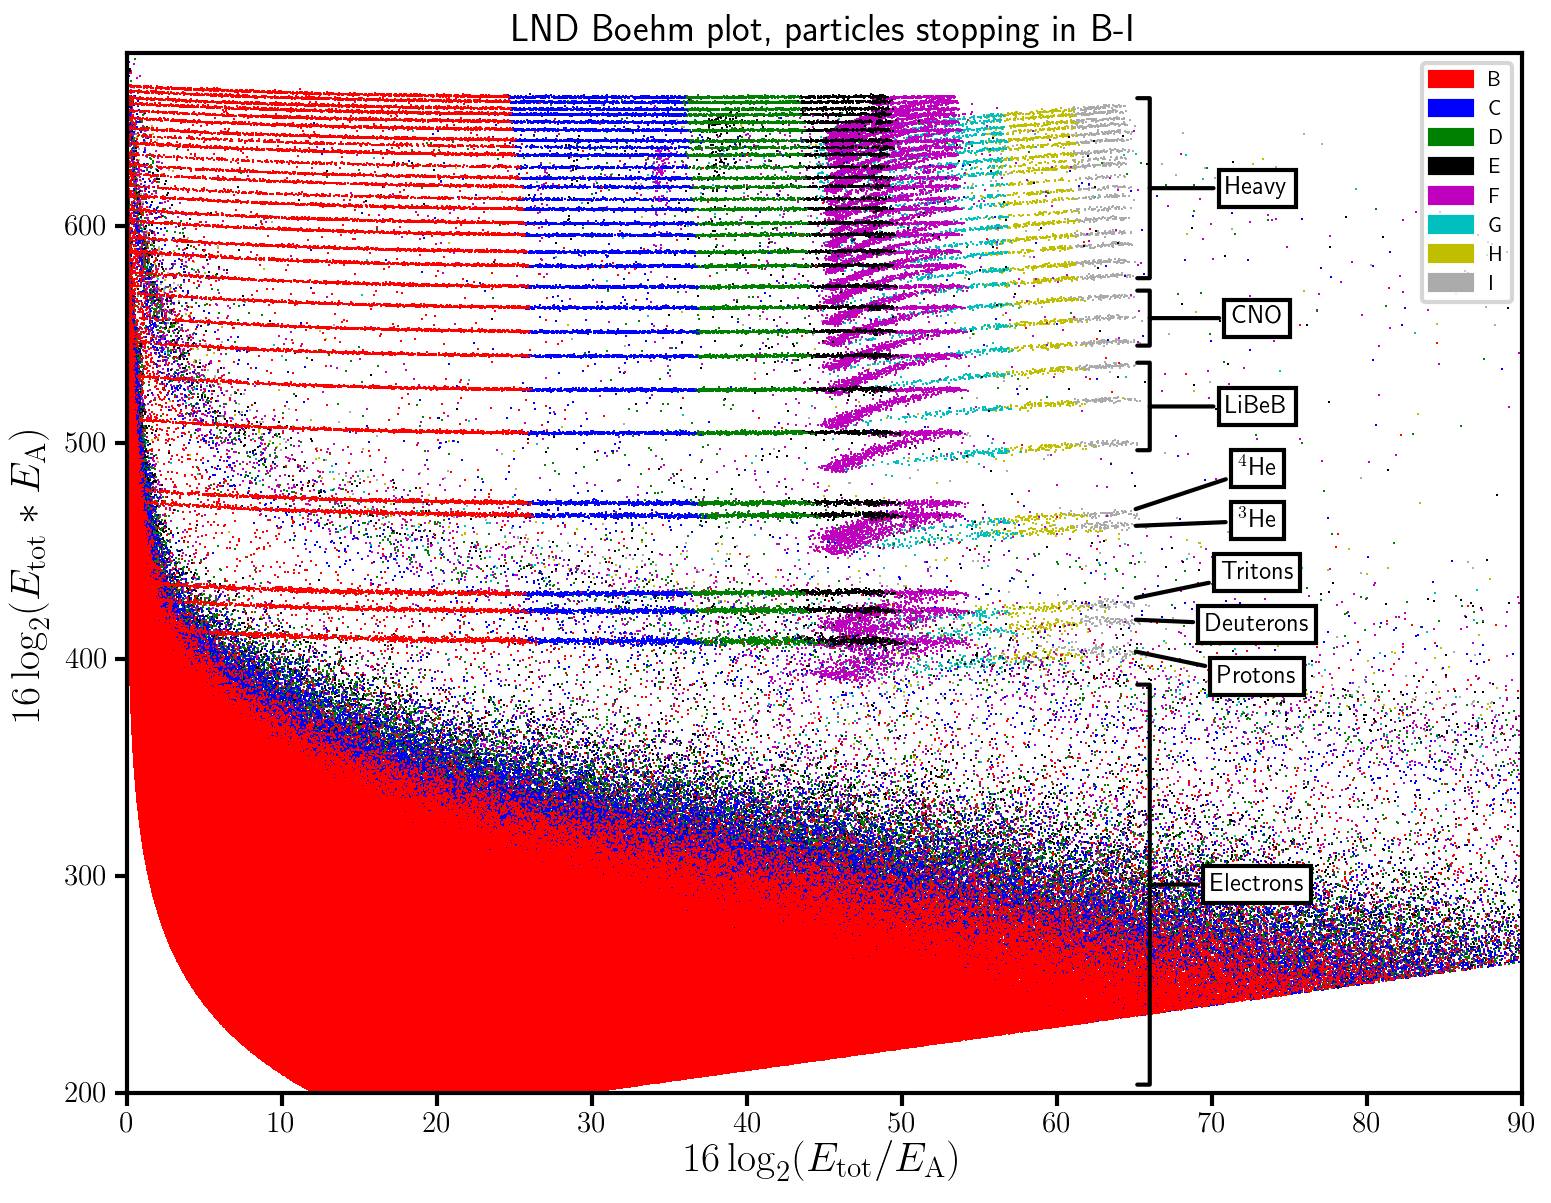
\includegraphics[width=0.8\textwidth]{images/LND_Boehm_plot_isotropic_on_top_of_A_annotated.png}
    \caption[LND Boehm plot of stopping particles based on the simulated data]{The different particle species are well discriminated in this LND Boehm plot which is a scatter plot of the \ac{LND} simulation data generated by the \ac{Geant4} tools \citep{Agostinelli-2003}. During the simulation, an isotropic source is positioned above detector A.}
    \label{Fig:LND-Boehm-plot}
\end{figure}


\subsection*{LND as dosimeter and neutral telescope}

\ac{LND} measures the \ac{TID} in the inner B segment utilizing the energy deposition and corresponding energy spectrum. The inner segment of C, which is surrounded by the B, D, and C outer segment and in anti-coincidence with all other detector segments, is used to measure the neutral dose rate caused by both fast neutrons and $\gamma$-rays. The above two measurements are the primary data products of \ac{LND}. \ac{TID} and dose in C play important roles in assessing the radiation environment on the lunar surface. 


\ac{LND} employs the E/F, G/H pairs which clamp a Gd-foil, to measure the thermal neutron flux. The Gd-foil has a large cross-section for thermal neutrons, resulting in a high probability of interaction with neutrons \citep{Wimmer2020SSRv}. After the capture of thermal neutrons in the Gd-foil, X-rays with energies of 43 keV and electrons with energies of 71 keV, 131 keV, and 173 keV are emitted and then detected by detectors closed to the foil.
In the calibration experiment, \ac{LND} successfully measured neutrons by calculating the energy spectrum discrepancy between E (G) and F (H) for neutrons coming from the front (back).
However, in actual measurements, the quality of the thermal neutron data is unexpectedly low due to various factors. The most prominent factors are the neutron background emitted from the \ac{RTG} and the \ac{RHU}. These radioactive sources generate heat to protect the lander and payload from the frozen night. But they also contribute significantly to the neutron background \citep{Zhang2020SciAdv}. Unfortunately, the direct measurement of the radiation sources had never been done, and only an experimental and empirical estimation of the contamination from the background on the data was conducted by \citet{Hou2020-LNDbackground}. Based on data from laboratory experiments and Monte Carlo simulations, \citet{Hou2020-LNDbackground} confirmed the non-negligible background interference and estimated the dose rate background. 

Another factor that affects the neutron measurements is the unanticipated noise increase in neutral channels F2 and H2. In those two channels, the single detector counter rates increased from about few thousands count/min to $10^6$ count/min, and energy spectra of noise channels indicate that the dominant energy of noise is below 300 keV. 
The high energy noise obscures the x-ray line at 43 keV and electron lines at 71 keV, 131 keV, and 173 keV, which are used to determine the thermal neutrons flux and make it more challenging to derive the accurate thermal neutron flux of lower intensity.
Furthermore, the larger count rates in those thermal neutron channels increase the dead time of counters. The dead time is the time during which the system is not able to record another event after one valid event \citep{leo1994techniques}. The increasing dead time of counters leads to the loss of valid events

Because thermal neutron measurements and neutron dose in C share the same counter buffer, the dead time issues also affect neutron dose in C. 

In H2 channel, the large amount of noise signals appeared simultaneous with the other noise channels since the third lunar day (see Sec.~\ref{sec:configuration_changes} and further discussion in chapter \ref{chp:LND_GCR_albedo}). While the increased noise level of F2 channel first appeared in the 17th lunar day, only lasting for few hours. Recently, the situation is becoming worse. The noisy period of F2 can account for about half of one lunar day during some days. In order to mitigate the dead time issue, we raise the corresponding threshold of 

noise detectors to a few hundred keV (depending on the noise level of each detector), resulting in the loss of the thermal neutrons data. The threshold of G2 and H1 has been raised 


The remaining data products related to dosimetric quantities that \ac{LND} provides are the \ac{LET} spectra. There are three types of \ac{LET} spectra in \ac{LND}'s normal data products - $ABC\bar{I}$, $\bar{A}BIJ$ and $ABIJ$. Those \ac{LET} spectra can be used to derive the quality factor (Q), which is a dimensionless modifier used in converting absorbed dose to to dose equivalent which is used to account for the biological effectiveness of different kinds of radiation \citep{Kerr1988Qualityfacgtor}.

%More details of the data products can be found in the instrument paper \citet{Wimmer2020SSRv}.

The first scientific results of \ac{LND} regarding the radiation environment on the lunar surface are reported by \citet{Zhang2020SciAdv}. These initial findings present the \ac{TID}, neutron dose, and \ac{LET} spectra of the first two lunar days. This represents the first-ever dynamic measurements of the radiation variation on the lunar surface. The average total absorbed dose rate in silicon is about 13.59$\pm$1.01 $\mu$Gy/hour. Amongst this total dose rate, the contribution from neutral particles is estimated to be $3.10 \pm 0.43 \mu$Gy/hour. These values are consistent with the measurements from the \ac{CRaTER} on \ac{LRO}.



\subsection*{Primary data products: Xmas plots}
\label{sec:xmas}

\begin{figure}
    \centering
    \includegraphics[width =0.95\textheight, height = 0.4\textheight, angle = 90]{images/xmas-2019-01-03To2022-11-29.png}
    \caption[\ac{LND} Xmas plot from measurements]{The completed Xmas plot (274 $\times$ 64) of \ac{LND} based on the measurements between 2019.1.3 and 2022.11.29. All the data products could be found in this matrix, including neutrals, \ac{LET} spectra, \ac{TID}, stopping and penetrating charged particles, including electrons, protons, helium nuclei and heavy ions. The corresponding simulation version can be found in \citet{Wimmer2020SSRv}}
    \label{Fig:measurement_Xmas}
\end{figure}

Fig.~\ref{Fig:measurement_Xmas} is the so-called "Xmas plot" \footnote{It was the front cover of the Xmas card of IEAP group in 2017. Hence we named it Xmas plot} of the \ac{LND}. The Xmas plot is an image of \ac{LND}'s memory space shaped in a 274 $\times$ 64 matrix, where each pixel in the Xmas plot servers as a counter. When \ac{LND} register a valid particle signal belong to some counters, the values of those counters will be incremented by one. 

Rules to determine which counter should be incremented are based on the deposited energy of particles in different detectors and are given in \citet{Wimmer2020SSRv}. The whole process are done onboard and the data are stored in the memory space of \ac{LND}.
In principle, all data products of \ac{LND} are extracted from this matrix. 
 

Unlike the simulated plot in \citet{Wimmer2020SSRv}, here we showcase a Xmas plot from the actual measurements between 2019.1.3 to 2022.11.29, encompassing all the data accumulated since the first lunar day observed by \ac{LND}. The green rows are the memory spaces that are not transmitted to ground in order to save telemetry bandwidth. 
For a more detailed explanation of the format of the Xmas plot, see \citet{Wimmer2020SSRv}.


\ac{LND} provides multiple data products including charged and neutral particle dose rate measured in silicon detectors, \ac{LET} spectra and neutral spectra, count rates of thermal neutrons, ion and electron flux variation and their energy spectra.

%The major different compared with the Xmas plot in \citep{Wimmer2020SSRv} is that LND measure not only the particle incident from above but also the albedo particles moving upward, while in the simulation, we did add the albedo component. It is obvious that in the penetrating panel of Xmas plot,  a higher than backgrond branch strech from middle to the left side. This branch represents the protons moving upward with enough energy fully penetrating all the detectors as well as the extra shielding from the lander structure. More details of how to derive albedo proton flux are given in Section.~\ref{sec:albedo_proton}.

\subsection*{Configuration changes of LND}
\label{sec:configuration_changes}
It is important to highlight that several configuration changes have been made after \ac{LND} was delivered and launched. Those configuration changes are reflected in 14 extra commands, which are uploaded to the control unit of \ac{LND} every morning of the lunar day, fixing software issues and malfunction issues. One of the software issues arises from errors in the software pipeline where the control unit uses the wrong channels to determine particle energies. Another one is due to the mistakes we made in simulations when designing data products, causing the location of the \ac{dps} boxes to shift in the X-mas plot, which is a matrix storing \ac{LND} data products (See below and \citet{Wimmer2020SSRv} for more details about the X-mas plot). Neverthless, the impact of the second problem on the data products is minor. 

The significant changes in the data products are mainly caused by raising the thresholds of channels which have turned noisy due to unforeseen thermal stresses, as well as to the fact that we had to disble the A2 channel. A2 represents the outer segment of the front detector A (see Appendix in chapter ~\ref{chp:LND_GCR_albedo} for more details of the changes). These changes are motivated by high observed noise levels in detectors A, H, I and J, which appeared coincidentally with the malfunction of the front lid. The front lid of \ac{LND} is a part of the lander and is designed to protect the fragile detectors inside the \ac{SH}. The lid is opened up to allow unobstructed measurements of the particles during lunar days and is closed immediately after the instrument is switched off, protecting the detectors from the extreme temperature decrease on the lunar surface and the lunar night. However, on the 3rd and 4th lunar days, \ac{LND} was switched off for a short period during working time, but the lid was left open. Though temperature on the lunar surface increased as the Sun rose, \ac{LND} and its detectors kept losing heat. Hence the temperature of the \ac{SH} dropped drastically, resulting in irreversible deformation of carriers and the attached detectors, particularly the detectors A and I/J in the front side and the bottom side. Consequently, the noise level increased significantly from below 20 kev to $\sim$ 10 - 200 keV) experienced a significant increase.

By implementing the changes mentioned above, we have successfully reduced the influence of those additional noise and mitigated their impact on the primary data products such as \ac{LET} spectra. However, it is worth noting that these changes still resulted in significant consequences for several other data products. For instance, we partly lose the measurement of \acp{MIP}, whose mean energy loss in the detectors is close to minimum, after the increment of the threshold of the I detector; the geometry factors of two \ac{LET} spectra and penetrating particle are reduced dramatically after disabling the A2 channel, which plays a key role in \ac{LND}'s measurement. For a better understanding of the configuration changes and their impact on the data products, see the appendix of chapter \ref{chp:LND_GCR_albedo}.
%The corresponding changes of the original code in the LND data processing pipeline are given in the appendix ~\ref{chp:appendix_LND_data_process_pipeline}.

\section {Solar orbiter and High energy telescope}
\label{sec:Solar_Orbiter}
Successfully launched on February 10, 2020, the \ac{SolO} mission \citep{Mueller-2020-SolO} is an international mission in coorperation between \ac{ESA} and \ac{NASA} with the aim to understand the Sun and how it controls the heliosphere. As indicated in the mission paper, the following scientific questions will be answered and further studied: (a). What drives the solar wind, and where does the coronal magnetic field originate from? (b). How do solar transients drive heliospheric variability? (c). How do solar eruptions produce the energetic particle radiation that fills the heliosphere? (d). How does the solar dynamo work and drive connections between the Sun and the heliosphere?

%After finishing the cuise phase which started at June 14, 2020, \ac{SolO} has been operating in the nominla mission phase since November 26, 2021 as scheduled.

\ac{SolO} has an elliptic heliocentric orbit with a closest perihelion of 0.29 AU (about 42$\times10^6$ km). Using several gravity assist maneuvers (Venus flybys and the Earth flybys), the orbit of \ac{SolO} will gradually tilt away from the ecliptic plane and, at the end of the nominal mission, will be 24 degrees above the Sun's equator. As of May 2023, \ac{SolO} is following an elliptical orbit circling the Sun, with a maximum solar latitude of 8.66 degrees. \ac{SolO} has finished five perihelia with the closest distance of 0.292 AU on September 3, 2022, and has started its 6th orbit, moving away from the Sun. Benefiting from the unique position of \ac{SolO} during this trip, the multiple scientific instruments onboard the \ac{SolO} can further advance our understanding of the Sun and its effects on the heliosphere. The evolution of distance of \ac{SolO} to the Sun and solar latitude of \ac{SolO} from 2020 to 2023 are given in Fig.~\ref{figL:SOLO_orbit_muller}.
\begin{figure}[ht]
    \centering
    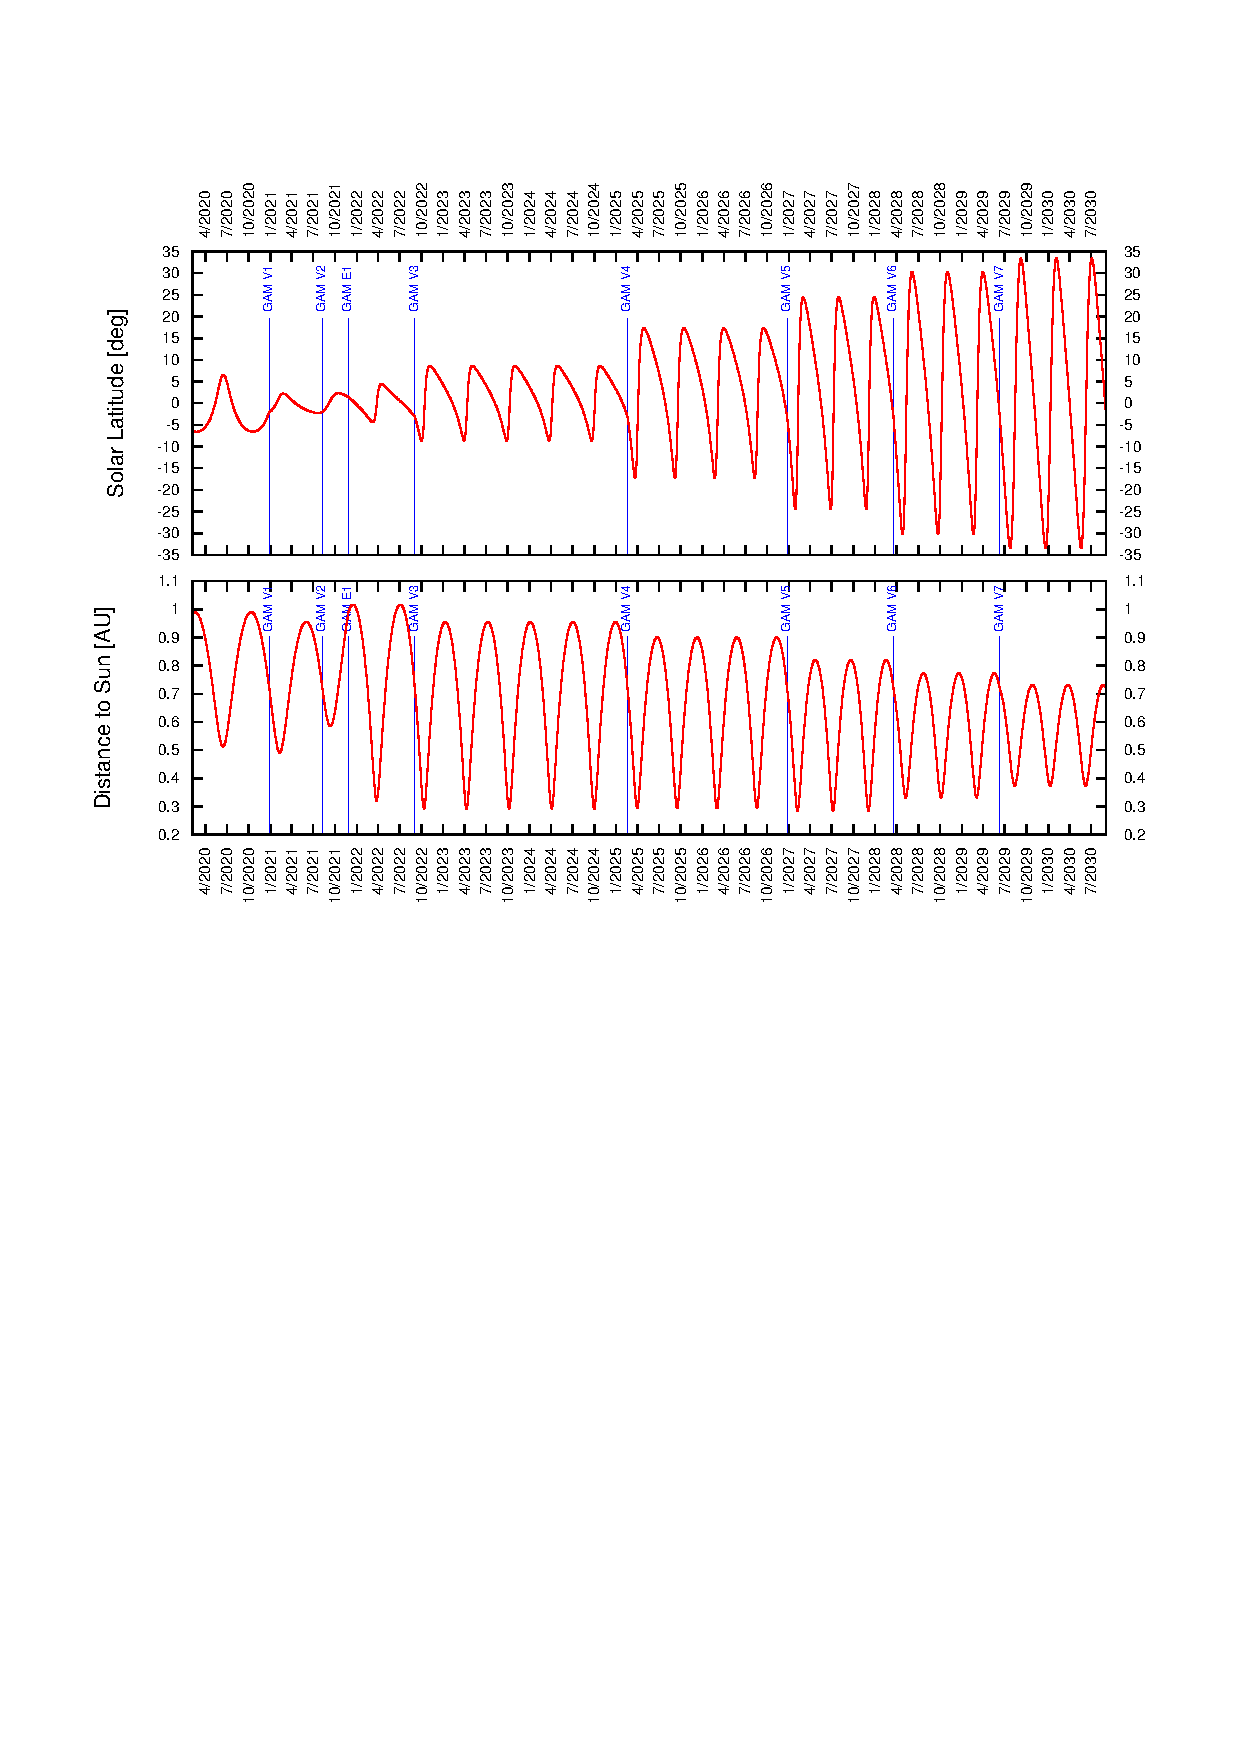
\includegraphics[width=0.8\textwidth]{images/Muller2020-fig28.pdf}
    \caption[The orbit of \ac{SolO} between 2020-2030]{The orbit of \ac{SolO} from 2020 to 2023. The figure is reproduced from \citet{Mueller-2020-SolO}.}
    \label{figL:SOLO_orbit_muller}
\end{figure}
%Three time Venus flyby happened on December 27, 2020, August 9, 2021 and September 4, 2022. The Earth GAM happend on Now 27, 2021.
%The above mentioned solo tragjectory information is taken from the Solar orbiter Consolidated Report on Mission analysis \footnotes{\url{https://issues.cosmos.esa.int/solarorbiterwiki/display/SOSP/Trajectory+Overview+-+10+February+2020+Launch}}

%in the relative field for instance the questions regarding solar coronal, solar magnetic field, solar wind, \ac{SEP}.
The \ac{EPD} \citep{RodriguezPacheco-2019-EPD} is part of the scientific payload onboard \ac{SolO}, measuring energetic particles over a large scale from few kev to GeV. The spectra, composition, time variations and directional distributions can be obtained and derived.
\ac{EPD} is comprises of four different sensors, the \ac{SIS}, the \ac{STEP}, the \ac{EPT} and the \acl{HET}. 
\ac{SIS} is a time-of-flight mass spectrometer that measures ion composition from $\sim$ 0.1 - few MeV nucleon$^{-1}$. \ac{STEP} measures electrons and ions with lower energies between 4 keV and 80 keV. The special design of \ac{STEP} allows it to have high pitch-angle resolution.
\ac{EPT} and \ac{HET} share the same electronics, and they are composed of two identical sensor units that are mounted perpendicularly on \ac{SolO}. This configuration enables the detection of the particle incident from four different directions. \ac{EPT} is designed to measure medium-energy electrons (ions)within an energy range of 25 keV - 400 keV (25keV - $\sim$ 6000 keV), while \ac{HET} completes the higher energy end, measuring electrons from 300 keV to 30 MeV and ions from 6.8 Mev/nuc to $\sim$ 100 MeV/nuc in the nominal data products. Notably, the penetrating data products of \ac{HET} extends the energy coverage of \ac{HET} up to $\sim$ 2 GeV/nuc \citep{Elftmann-2020-PhD}.
The full energy range of those four instruments for different particle species is given in Fig.~\ref{Fig:EPD-energy-coverage}.
In this section, we provide a brief introduction of \ac{HET}, which is the focus of the study in chapter \ref{chp:ACR_Helium}. More detailed information on the other components can be found in the instrument paper \citep{RodriguezPacheco-2019-EPD} and the first years' overview paper of \ac{EPD} \citep{Wimmer2021AA}.


\begin{figure}
    \centering
    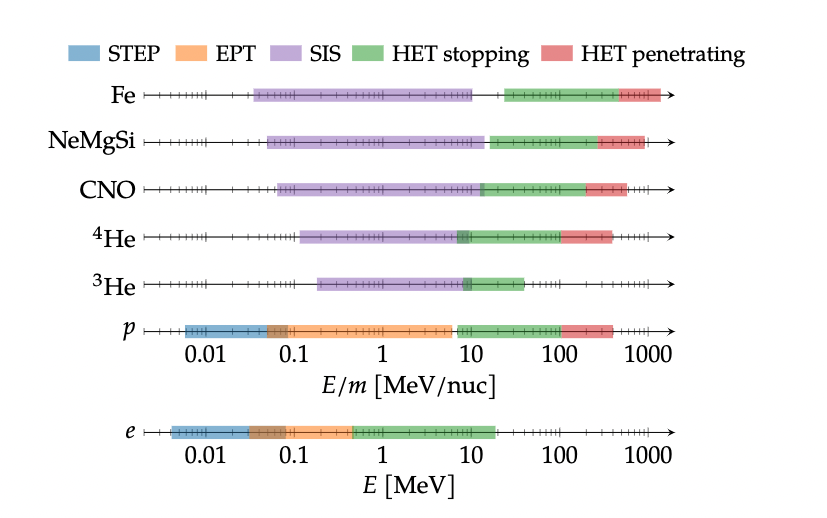
\includegraphics[width = \textwidth]{images/EPD_coverage.png}
    \caption[The energy coverage of different \ac{EPD} sensors]{The energy coverage of different \ac{EPD} sensors for different particle species. This figure is an updated energy coverage plot made by \citet{JohanPhd2020}, based on a similar plot from \citet{RodriguezPacheco-2019-EPD}. The HET measurements are split into stopping and penetrating parts, and the latter one considerably extends \ac{HET}'s capability \citep{Elftmann-2020-PhD}.}
    \label{Fig:EPD-energy-coverage}
\end{figure}  

\subsection*{High Energy Telescope (HET)}

\begin{figure}
    \centering
    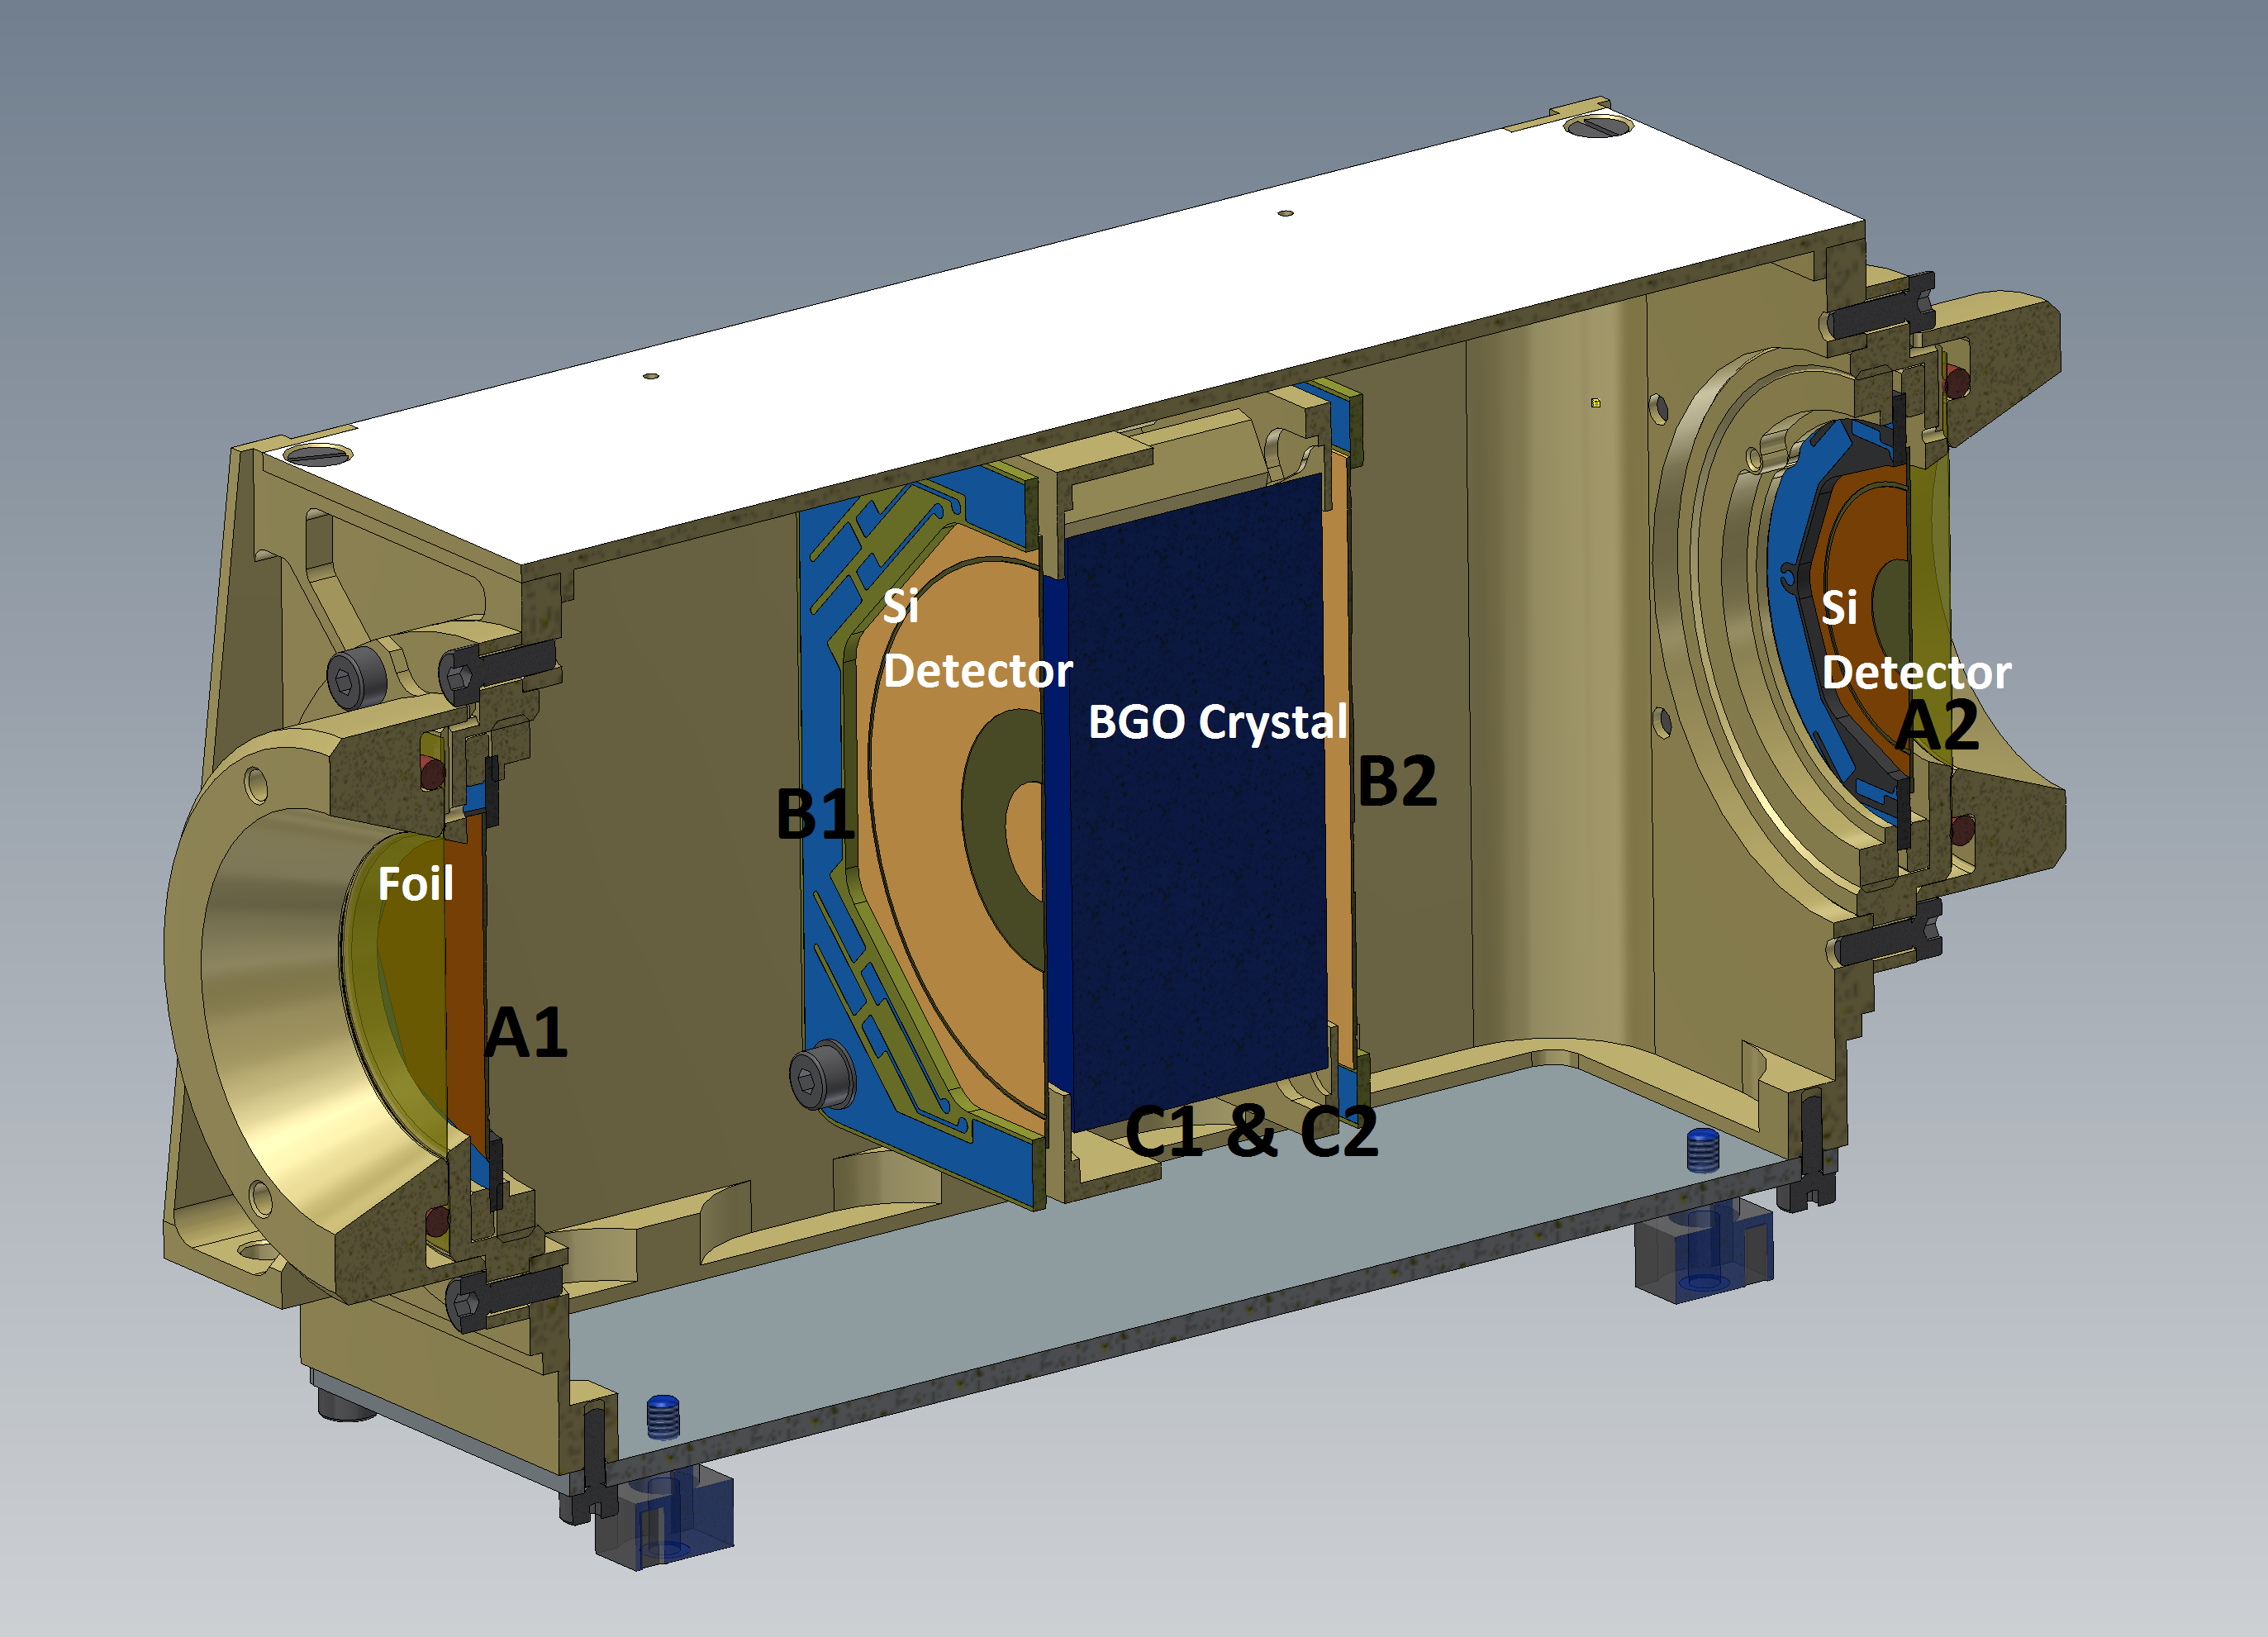
\includegraphics[width = \textwidth]{images/het.png}
    \caption[Cut view of \ac{HET} sensor head]{Cut view of \ac{HET} sensor head. The corresponding detector names are labeled. This figure is reproduced from \citet{RodriguezPacheco-2019-EPD}.}
    \label{fig:HET-sensor-head}
\end{figure}

A cut view of the \ac{HET} sensor head is depicted in Fig.~\ref{fig:HET-sensor-head}. \ac{HET} is a double-ended telescope. The sensor head of \ac{HET} consists of four 300 $\mu$m silicon \ac{SSD} stacks, with two on each side (A1, B1 on the front side and A2, B2 on the back side) and a 2-cm thick \ac{BGO} ($Bi_{4}Ge_{3}O_{12}$) scintillator which is named as detector C in the center. The sensor head setup is similar to the configuration of the \ac{RAD} \citep{Hassler-2012-MSLRAD}, another instrument developed by Kiel Univeristy, which is currently operating on the Martian surface.  

\ac{HET} uses the $\mathrm{dE/dX - E}$ technique to discriminate different particle species of different energy. This method is the same as the measurement principle of \ac{LND} that has been well explained before. The particle species that \ac{HET} can discriminate include electrons, protons, helium nuclei, and all heavy ions such as carbon, nitrogen, oxygen, and iron.  

Once the charged particle hit and penetrate the A detector (A1 or A2), they can be split into stopping particles and penetrating particles, depending on their energy and whether they stop in detector B/C. As given in Table 22 of \citet{RodriguezPacheco-2019-EPD}, the corresponding nominal data products are ABnC, which corresponds to ions stopping in B with the energy of 6.5 - 9.5 Me/nuc, ABC, which register ions stopping in C with an energy range of $\sim$10 - $\sim$ 100 MeV/nuc, and penetrating detector C with energy above 100 MeV/nuc up to $\sim$ 2 GeV.

%For the penetrating particle, their primary energy can be estimated based on the energy loss on the detector and the \ac{Geant4} simulation. The aforementioned nominal data products of HET contribute to the study of \ac{SEP}, \ac{ACR}, and \ac{GCR}.


In addition to the nominal charged particle data products, it is important to emphasize the significant contribution of housekeeping data in our studies. Housekeeping data include temperature, voltage, current, single/multiple detector count rate.  
They have the highest priority for downlinking to the Earth and are used to monitor the instrument status and health. Here, what we emphasize is mainly the single detector count rate. Although the single detector count rates are not designed for scientific purposes, they still provide valuable insight into the instrument performance, and their contributions to the scientific studies is impressive \citep{Wimmer2021AA}, especially the counter rate from the \ac{BGO} scintillator crystal (C detector). 

This counter does not require any coincidence condition and responds to particles from all directions and types. The sole requirement is that the deposited energy exceeds the threshold of the C detector. Due to its large geometry factor, this counter exhibits excellent counting statistics and can be used to detect minor disturbances in the \ac{GCR} background. For example, \citet{Forstner-2021-SolO} use this counter to study a \ac{FD} with an amplitude of 3\% when a \ac{CME} passed \ac{SolO} on April 19, 2020. In addition, \citet{Allen2021AA_venus} found an $\sim$ 5\% drop in the count rates during the first Venus flyby. This drop is due to the blockage by the planetary body  on \ac{FOV} of \ac{HET}.

% Similar to the single detector count rate, we also utilize the L2 counters named \textit{any(a1, b1)} or \textit{any(a2,b2)} to determine the periods of \acp{SEP}. The counters sum up every signal that triggers detectors A1 (A2) and B1 (B2) in the sensor head, regardless of the primary energy and the particle species. \acp{GCR}, which are slowly varying, are the dominant particles in the background of this counter. Therefore, a temporal increase indicates an incoming of \ac{SEP} event. These data products exhibit better counting statistics than the nominal science data products, which are designed to derive the flux. Additionally, \textit{any(a1, b1)} or \textit{any(a2,b2)} are more sensitive to lower energy particles from \acp{SEP}, as they have a lower energy threshold of $\sim$ 50 keV compared to the C counter \citep{Elftmann-2020-PhD}. The counters can detect electrons and ions with energy below 1 MeV. As a result, those two counters are particularly useful in determining the start and end time of the \ac{SEP} events, no matter what particles trigger them. In chapter \ref{chp:ACR_Helium}, where we are interested in \acp{ACR}, we remove \ac{SEP} time periods determined by this method based on the \textit{any(a1,b1)} counter to enable an accurate \ac{ACR} measurement.


For more details on the inner structure and parameters of the \ac{HET}, as well as the most updated status of \ac{HET}, one could refer to \citet{Elftmann-2020-PhD, RodriguezPacheco-2019-EPD, Wimmer2021AA}.

